% Options for packages loaded elsewhere
\PassOptionsToPackage{unicode}{hyperref}
\PassOptionsToPackage{hyphens}{url}
%
\documentclass[
]{article}
\usepackage{lmodern}
\usepackage{amsmath}
\usepackage{ifxetex,ifluatex}
\ifnum 0\ifxetex 1\fi\ifluatex 1\fi=0 % if pdftex
  \usepackage[T1]{fontenc}
  \usepackage[utf8]{inputenc}
  \usepackage{textcomp} % provide euro and other symbols
  \usepackage{amssymb}
\else % if luatex or xetex
  \usepackage{unicode-math}
  \defaultfontfeatures{Scale=MatchLowercase}
  \defaultfontfeatures[\rmfamily]{Ligatures=TeX,Scale=1}
\fi
% Use upquote if available, for straight quotes in verbatim environments
\IfFileExists{upquote.sty}{\usepackage{upquote}}{}
\IfFileExists{microtype.sty}{% use microtype if available
  \usepackage[]{microtype}
  \UseMicrotypeSet[protrusion]{basicmath} % disable protrusion for tt fonts
}{}
\makeatletter
\@ifundefined{KOMAClassName}{% if non-KOMA class
  \IfFileExists{parskip.sty}{%
    \usepackage{parskip}
  }{% else
    \setlength{\parindent}{0pt}
    \setlength{\parskip}{6pt plus 2pt minus 1pt}}
}{% if KOMA class
  \KOMAoptions{parskip=half}}
\makeatother
\usepackage{xcolor}
\IfFileExists{xurl.sty}{\usepackage{xurl}}{} % add URL line breaks if available
\IfFileExists{bookmark.sty}{\usepackage{bookmark}}{\usepackage{hyperref}}
\hypersetup{
  pdftitle={Visualisation of the wind energy power plant repowering potential in Rhineland Palatinate with R using Leaflet and Shiny},
  pdfauthor={Kelly Lasisi, Anja Weiler, Elias Cuadra},
  hidelinks,
  pdfcreator={LaTeX via pandoc}}
\urlstyle{same} % disable monospaced font for URLs
\usepackage[margin=1in]{geometry}
\usepackage{color}
\usepackage{fancyvrb}
\newcommand{\VerbBar}{|}
\newcommand{\VERB}{\Verb[commandchars=\\\{\}]}
\DefineVerbatimEnvironment{Highlighting}{Verbatim}{commandchars=\\\{\}}
% Add ',fontsize=\small' for more characters per line
\usepackage{framed}
\definecolor{shadecolor}{RGB}{248,248,248}
\newenvironment{Shaded}{\begin{snugshade}}{\end{snugshade}}
\newcommand{\AlertTok}[1]{\textcolor[rgb]{0.94,0.16,0.16}{#1}}
\newcommand{\AnnotationTok}[1]{\textcolor[rgb]{0.56,0.35,0.01}{\textbf{\textit{#1}}}}
\newcommand{\AttributeTok}[1]{\textcolor[rgb]{0.77,0.63,0.00}{#1}}
\newcommand{\BaseNTok}[1]{\textcolor[rgb]{0.00,0.00,0.81}{#1}}
\newcommand{\BuiltInTok}[1]{#1}
\newcommand{\CharTok}[1]{\textcolor[rgb]{0.31,0.60,0.02}{#1}}
\newcommand{\CommentTok}[1]{\textcolor[rgb]{0.56,0.35,0.01}{\textit{#1}}}
\newcommand{\CommentVarTok}[1]{\textcolor[rgb]{0.56,0.35,0.01}{\textbf{\textit{#1}}}}
\newcommand{\ConstantTok}[1]{\textcolor[rgb]{0.00,0.00,0.00}{#1}}
\newcommand{\ControlFlowTok}[1]{\textcolor[rgb]{0.13,0.29,0.53}{\textbf{#1}}}
\newcommand{\DataTypeTok}[1]{\textcolor[rgb]{0.13,0.29,0.53}{#1}}
\newcommand{\DecValTok}[1]{\textcolor[rgb]{0.00,0.00,0.81}{#1}}
\newcommand{\DocumentationTok}[1]{\textcolor[rgb]{0.56,0.35,0.01}{\textbf{\textit{#1}}}}
\newcommand{\ErrorTok}[1]{\textcolor[rgb]{0.64,0.00,0.00}{\textbf{#1}}}
\newcommand{\ExtensionTok}[1]{#1}
\newcommand{\FloatTok}[1]{\textcolor[rgb]{0.00,0.00,0.81}{#1}}
\newcommand{\FunctionTok}[1]{\textcolor[rgb]{0.00,0.00,0.00}{#1}}
\newcommand{\ImportTok}[1]{#1}
\newcommand{\InformationTok}[1]{\textcolor[rgb]{0.56,0.35,0.01}{\textbf{\textit{#1}}}}
\newcommand{\KeywordTok}[1]{\textcolor[rgb]{0.13,0.29,0.53}{\textbf{#1}}}
\newcommand{\NormalTok}[1]{#1}
\newcommand{\OperatorTok}[1]{\textcolor[rgb]{0.81,0.36,0.00}{\textbf{#1}}}
\newcommand{\OtherTok}[1]{\textcolor[rgb]{0.56,0.35,0.01}{#1}}
\newcommand{\PreprocessorTok}[1]{\textcolor[rgb]{0.56,0.35,0.01}{\textit{#1}}}
\newcommand{\RegionMarkerTok}[1]{#1}
\newcommand{\SpecialCharTok}[1]{\textcolor[rgb]{0.00,0.00,0.00}{#1}}
\newcommand{\SpecialStringTok}[1]{\textcolor[rgb]{0.31,0.60,0.02}{#1}}
\newcommand{\StringTok}[1]{\textcolor[rgb]{0.31,0.60,0.02}{#1}}
\newcommand{\VariableTok}[1]{\textcolor[rgb]{0.00,0.00,0.00}{#1}}
\newcommand{\VerbatimStringTok}[1]{\textcolor[rgb]{0.31,0.60,0.02}{#1}}
\newcommand{\WarningTok}[1]{\textcolor[rgb]{0.56,0.35,0.01}{\textbf{\textit{#1}}}}
\usepackage{graphicx}
\makeatletter
\def\maxwidth{\ifdim\Gin@nat@width>\linewidth\linewidth\else\Gin@nat@width\fi}
\def\maxheight{\ifdim\Gin@nat@height>\textheight\textheight\else\Gin@nat@height\fi}
\makeatother
% Scale images if necessary, so that they will not overflow the page
% margins by default, and it is still possible to overwrite the defaults
% using explicit options in \includegraphics[width, height, ...]{}
\setkeys{Gin}{width=\maxwidth,height=\maxheight,keepaspectratio}
% Set default figure placement to htbp
\makeatletter
\def\fps@figure{htbp}
\makeatother
\setlength{\emergencystretch}{3em} % prevent overfull lines
\providecommand{\tightlist}{%
  \setlength{\itemsep}{0pt}\setlength{\parskip}{0pt}}
\setcounter{secnumdepth}{-\maxdimen} % remove section numbering
\ifluatex
  \usepackage{selnolig}  % disable illegal ligatures
\fi

\title{Visualisation of the wind energy power plant repowering potential
in Rhineland Palatinate with R using Leaflet and Shiny}
\author{Kelly Lasisi, Anja Weiler, Elias Cuadra}
\date{10 4 2021}

\begin{document}
\maketitle

{
\setcounter{tocdepth}{4}
\tableofcontents
}
\hypertarget{introduction}{%
\subsubsection{1. Introduction}\label{introduction}}

The project ``Municipal greenhouse gas accounting and regional climate
protection portals in Rhineland-Palatinate (KomBiReK)'', funded by the
European Regional Development Fund (EFRE) and the State of
Rhineland-Palatinate supports the creation of municipal climate
protection measures in order to achieve the climate protection goals of
the municipalities and the state and thereby increase regional added
value, ensure sustainability and thus improve the quality of life of all
citizens. When developing municipal climate protection, a sound strategy
is required with regard to the legally anchored striving for climate
neutrality in the state of Rhineland-Palatinate (LKSG paragraph 4,
2014). The energy transition is a cornerstone of this strategy and
Rhineland-Palatinate wants to play a pioneering role in the
implementation of the energy transition. With this in mind, the state
government publishes on its website that Rhineland-Palatinate will cover
100\% of its electricity needs from renewable energies by 2030. In
addition to energy from the sun, water and biomass, two thirds of the
electricity generated in 2030 should come from wind power and is
therefore the subject of the following considerations (state government
Rhineland-Palatinate, 2021).

There are two ways of increasing the amount of electricity generated by
wind energy. On the one hand, areas that are still available can be
identified and built on with new wind energy power plants (WEPP). On the
other hand, existing old WEPP with low electricity fed in, can be
replaced by new and more efficient systems through what is known as
``repowering''. To identify, compare and visualise the old WEPP in
Rhineland-Palatinate that could be potentially suitable for a repowering
is the task of this work. To accomplish this goal the necessary data
needs to be prepared followed by a visualisation process with Leaflet
and finally an interactive Shiny application will allow to select
different date ranges and search and find WEPP and their related
technical information and the repowering potential that could be
achieved.

\hypertarget{software-and-data}{%
\subsubsection{2. Software and Data}\label{software-and-data}}

For the data wrangling and processing as well as the creation of the
application R version 4.0.3 (2020-10-10) -- ``Bunny-Wunnies Freak Out''
and RStudio Version 1.3.1093 was used.

\hypertarget{data-from-the-transmission-system-operator-amprion-and-the-market-master-data-register-mastr}{%
\paragraph{2.1 Data from the transmission system operator Amprion and
the market master data register
(MaStR)}\label{data-from-the-transmission-system-operator-amprion-and-the-market-master-data-register-mastr}}

The data originated partly from a dataset of the transmission network
operator Amprion from 2019 (\url{https://www.amprion.net/}), responsible
for Rhineland-Palatinate. These consist of system master data including
energy source, system type, performance, date of commissioning, system
key and movement data including amount of electricity fed in and
remuneration of each wind energy power plant in Rhineland-Palatinate.
The second source is an abstract, taken in October 2020, of the market
master data register (Marktstammdatenregister (MaStR),
\url{https://www.marktstammdatenregister.de/MaStR}) maintained by the
Federal Network Agency since the beginning of 2017. In general, all
active systems connected to the grid for generating electricity or gas
plus the market players involved must be registered here. Important
information on the place, the municipality, technical information and,
above all, the EEG (Renewable Energy Act) system key in combination with
the geo-reference of all registered WEPP in Rhineland-Palatinate can be
viewed in the MaStR. Since the dataset of Amprion does not have certain
variables which the abstract of the MaStR has, these two datasets were
compiled, processed and merged together by the EEG system key by the
Energy Agency of Rhineland-Palatinate. The processing included a
calculation of the full load hours, electricity yield in 2019,
electricity yield after repowering, the increase of electricity yield in
percent through repowering, emission reduction given the emission factor
of the federal electricity mix in 2019 and then an addition to the
previously created data table. Thus, the used data was provided as a csv
file with the name msb19\_new.csv including the described information of
1750 WEPPs out of which 416 WEPP had incorrect or missing geographical
references.

\hypertarget{data-preparation}{%
\paragraph{2.2 Data preparation}\label{data-preparation}}

To create a geographical reference for all WEPP the geocode\_OSM
function was uses to find the WEPP according to their address. Because
there was a lot of data wrangling and iterative processing, the
extensive code is not displayed in this report but for the purpose of
reproducibility it is to be found in the original rmarkdown file
(repowering\_report.Rmd) also the coding blocks can be seen
\href{rscripts//repowering_data_preparation.R}{\textbf{here}}. After
filtering for the WEPP that were built before 2006, seven WEPP still
remained without geographical reference. This generated data frame was
then saved as msb19\_before2005\_geocoded.csv and was the basis for the
further usage in the Leaflet map and the Shiny application.

\hypertarget{creation-of-a-leaflet-map-of-wepp-in-rhineland-palatinate-built-before-2006}{%
\paragraph{2.3 Creation of a Leaflet map of WEPP in Rhineland-Palatinate
built before
2006}\label{creation-of-a-leaflet-map-of-wepp-in-rhineland-palatinate-built-before-2006}}

In order to build an interactive application a Leaflet map with the
described dataset is created first. The visualisation consists of the
OpenStreetMap maptiles, a marker for every WEPP with cluster options and
the borders of the state county and municipalities which can be switched
on and off. The code to generate the map as well as a link to the
interactive map is provided below.

\textbf{To the repowering map}

\begin{Shaded}
\begin{Highlighting}[]
\DocumentationTok{\#\#\#\#\#\#\#\#\#\#\#\#\#\#\#\#\#\#\#\#\#\#\#\#\#\#\#\#\#\#\#\#\#\#\#\#\#\#\#\#\#\#\#\#\#\#\#\#\#\#\#\#\#\#\#\#\#\#\#\#\#\#\#\#\#\#\#\#\#\#\#\#\#\#\#\#\#\#\#}
\CommentTok{\#load packages and import data                                                \#}
\DocumentationTok{\#\#\#\#\#\#\#\#\#\#\#\#\#\#\#\#\#\#\#\#\#\#\#\#\#\#\#\#\#\#\#\#\#\#\#\#\#\#\#\#\#\#\#\#\#\#\#\#\#\#\#\#\#\#\#\#\#\#\#\#\#\#\#\#\#\#\#\#\#\#\#\#\#\#\#\#\#\#\#}
\FunctionTok{Sys.setenv}\NormalTok{(}\AttributeTok{LANG =} \StringTok{"en"}\NormalTok{)}
\NormalTok{pacman}\SpecialCharTok{::}\FunctionTok{p\_load}\NormalTok{(rio, data.table, tidyverse, tidyr, purrr, magrittr, compare, }
\NormalTok{               ggplot2, leaflet, sp, raster, rgdal, ggmap, htmltools, }
\NormalTok{               htmlwidgets, tmaptools)}
\NormalTok{msb19\_before2005\_geocoded }\OtherTok{\textless{}{-}} \FunctionTok{read.csv}\NormalTok{(}\StringTok{"data//msb19\_before2005\_geocoded.csv"}\NormalTok{, }
                                      \AttributeTok{header=}\ConstantTok{TRUE}\NormalTok{)}
\DocumentationTok{\#\#\#\#\#\#\#\#\#\#\#\#\#\#\#\#\#\#\#\#\#\#\#\#\#\#\#\#\#\#\#\#\#\#\#\#\#\#\#\#\#\#\#\#\#\#\#\#\#\#\#\#\#\#\#\#\#\#\#\#\#\#\#\#\#\#\#\#\#\#\#\#\#\#\#\#\#\#\#}
\CommentTok{\#change leistung\_s to numeric and indatum\_s to date}
\DocumentationTok{\#\#\#\#\#\#\#\#\#\#\#\#\#\#\#\#\#\#\#\#\#\#\#\#\#\#\#\#\#\#\#\#\#\#\#\#\#\#\#\#\#\#\#\#\#\#\#\#\#\#\#\#\#\#\#\#\#\#\#\#\#\#\#\#\#\#\#\#\#\#\#\#\#\#\#\#\#\#\#}
\NormalTok{msb19\_before2005\_geocoded}\SpecialCharTok{$}\NormalTok{leistung\_s }\OtherTok{\textless{}{-}} \FunctionTok{as.numeric}\NormalTok{(msb19\_before2005\_geocoded}\SpecialCharTok{$}
\NormalTok{                                                     leistung\_s)}
\NormalTok{msb19\_before2005\_geocoded}\SpecialCharTok{$}\NormalTok{indatum\_s }\OtherTok{\textless{}{-}} \FunctionTok{as.Date}\NormalTok{(msb19\_before2005\_geocoded}\SpecialCharTok{$}
\NormalTok{                                                 indatum\_s, }\StringTok{"\%Y{-}\%m{-}\%d"}\NormalTok{)}
\DocumentationTok{\#\#\#\#\#\#\#\#\#\#\#\#\#\#\#\#\#\#\#\#\#\#\#\#\#\#\#\#\#\#\#\#\#\#\#\#\#\#\#\#\#\#\#\#\#\#\#\#\#\#\#\#\#\#\#\#\#\#\#\#\#\#\#\#\#\#\#\#\#\#\#\#\#\#\#\#\#\#\#}
\CommentTok{\#load borders of Rhineland{-}Palatinate as shape files                          \#}
\DocumentationTok{\#\#\#\#\#\#\#\#\#\#\#\#\#\#\#\#\#\#\#\#\#\#\#\#\#\#\#\#\#\#\#\#\#\#\#\#\#\#\#\#\#\#\#\#\#\#\#\#\#\#\#\#\#\#\#\#\#\#\#\#\#\#\#\#\#\#\#\#\#\#\#\#\#\#\#\#\#\#\#}
\NormalTok{land }\OtherTok{\textless{}{-}} \FunctionTok{readOGR}\NormalTok{(}\StringTok{"Grenzen/Landesgrenze\_RLP.shp"}\NormalTok{)}
\NormalTok{landkreise }\OtherTok{\textless{}{-}} \FunctionTok{readOGR}\NormalTok{(}\StringTok{"Grenzen/Landkreise\_RLP.shp"}\NormalTok{)}
\NormalTok{gemeinden }\OtherTok{\textless{}{-}} \FunctionTok{readOGR}\NormalTok{(}\StringTok{"Grenzen/Verbandsgemeinde\_RLP.shp"}\NormalTok{)}
\DocumentationTok{\#\#\#\#\#\#\#\#\#\#\#\#\#\#\#\#\#\#\#\#\#\#\#\#\#\#\#\#\#\#\#\#\#\#\#\#\#\#\#\#\#\#\#\#\#\#\#\#\#\#\#\#\#\#\#\#\#\#\#\#\#\#\#\#\#\#\#\#\#\#\#\#\#\#\#\#\#\#\#}
\CommentTok{\#create map                                                                   \#}
\DocumentationTok{\#\#\#\#\#\#\#\#\#\#\#\#\#\#\#\#\#\#\#\#\#\#\#\#\#\#\#\#\#\#\#\#\#\#\#\#\#\#\#\#\#\#\#\#\#\#\#\#\#\#\#\#\#\#\#\#\#\#\#\#\#\#\#\#\#\#\#\#\#\#\#\#\#\#\#\#\#\#\#}
\NormalTok{m }\OtherTok{\textless{}{-}} \FunctionTok{leaflet}\NormalTok{(}\AttributeTok{data =}\NormalTok{ msb19\_before2005\_geocoded) }\SpecialCharTok{\%\textgreater{}\%}
  \FunctionTok{addTiles}\NormalTok{() }\SpecialCharTok{\%\textgreater{}\%}
  
  \FunctionTok{addPolygons}\NormalTok{(}\AttributeTok{data =}\NormalTok{ land,}
              \AttributeTok{color =} \StringTok{"\#5DADE2"}\NormalTok{,}
              \AttributeTok{weight =} \DecValTok{2}\NormalTok{,}
              \AttributeTok{opacity =} \FloatTok{0.6}\NormalTok{,}
              \AttributeTok{fillColor =} \StringTok{"\#5DADE200"}\NormalTok{,}
              \AttributeTok{highlight =} \FunctionTok{highlightOptions}\NormalTok{(}\AttributeTok{weight =} \DecValTok{7}\NormalTok{,}
                                           \AttributeTok{color =} \StringTok{"\#5DADE2"}\NormalTok{,}
                                           \AttributeTok{fillColor =} \StringTok{"\#5DADE2"}\NormalTok{,}
                                           \AttributeTok{fillOpacity =} \FloatTok{0.3}\NormalTok{,}
                                           \AttributeTok{bringToFront =} \ConstantTok{TRUE}\NormalTok{),}
              \AttributeTok{label =} \StringTok{"Rheinland{-}Pfalz"}\NormalTok{,}
              \AttributeTok{group =} \StringTok{"Rheinland{-}Pfalz"}\NormalTok{) }\SpecialCharTok{\%\textgreater{}\%} 
  
  \FunctionTok{addPolygons}\NormalTok{(}\AttributeTok{data =}\NormalTok{ landkreise,}
              \AttributeTok{color =} \StringTok{"\#000fff"}\NormalTok{,}
              \AttributeTok{weight =} \DecValTok{2}\NormalTok{,}
              \AttributeTok{opacity =} \FloatTok{0.6}\NormalTok{,}
              \AttributeTok{fillColor =} \StringTok{"\#000fff00"}\NormalTok{,}
              \AttributeTok{highlight =} \FunctionTok{highlightOptions}\NormalTok{(}\AttributeTok{weight =} \DecValTok{7}\NormalTok{,}
                                           \AttributeTok{color =} \StringTok{"\#000fff"}\NormalTok{,}
                                           \AttributeTok{fillColor =} \StringTok{"\#000fff"}\NormalTok{,}
                                           \AttributeTok{fillOpacity =} \FloatTok{0.3}\NormalTok{,}
                                           \AttributeTok{bringToFront =} \ConstantTok{TRUE}\NormalTok{),}
              \AttributeTok{label =}\NormalTok{ landkreise}\SpecialCharTok{$}\NormalTok{ldkreis,}
              \AttributeTok{group =} \StringTok{"Landkreise"}\NormalTok{) }\SpecialCharTok{\%\textgreater{}\%}
  
  \FunctionTok{addPolygons}\NormalTok{(}\AttributeTok{data =}\NormalTok{ gemeinden,}
              \AttributeTok{color =} \StringTok{"\#D93F0D"}\NormalTok{,}
              \AttributeTok{weight =} \DecValTok{1}\NormalTok{,}
              \AttributeTok{opacity =} \FloatTok{0.6}\NormalTok{,}
              \AttributeTok{fillColor =} \StringTok{"\#D93F0D00"}\NormalTok{,}
              \AttributeTok{highlight =} \FunctionTok{highlightOptions}\NormalTok{(}\AttributeTok{weight =} \DecValTok{7}\NormalTok{,}
                                           \AttributeTok{color =} \StringTok{"\#D93F0D"}\NormalTok{,}
                                           \AttributeTok{fillColor =} \StringTok{"\#D93F0D"}\NormalTok{,}
                                           \AttributeTok{fillOpacity =} \FloatTok{0.3}\NormalTok{,}
                                           \AttributeTok{bringToFront =} \ConstantTok{TRUE}\NormalTok{),}
              \AttributeTok{label =}\NormalTok{ gemeinden}\SpecialCharTok{$}\NormalTok{vgname,}
              \AttributeTok{group =} \StringTok{"Verbandsgemeinden"}\NormalTok{) }\SpecialCharTok{\%\textgreater{}\%} 
  \FunctionTok{addLayersControl}\NormalTok{(}\AttributeTok{overlayGroups =} \FunctionTok{c}\NormalTok{(}\StringTok{"Rheinland{-}Pfalz"}\NormalTok{, }\StringTok{"Landkreise"}\NormalTok{,}
                                     \StringTok{"Verbandsgemeinden"}\NormalTok{),}
                   \AttributeTok{options =} \FunctionTok{layersControlOptions}\NormalTok{(}\AttributeTok{collapsed =} \ConstantTok{FALSE}\NormalTok{)) }\SpecialCharTok{\%\textgreater{}\%} 
  \FunctionTok{addMarkers}\NormalTok{(}\AttributeTok{lng =}\NormalTok{ msb19\_before2005\_geocoded}\SpecialCharTok{$}\NormalTok{lon\_wgs84,}
             \AttributeTok{lat =}\NormalTok{ msb19\_before2005\_geocoded}\SpecialCharTok{$}\NormalTok{lat\_wgs84,}
             \AttributeTok{clusterOptions =} \FunctionTok{markerClusterOptions}\NormalTok{(}\AttributeTok{disableClusteringAtZoom =} \DecValTok{10}\NormalTok{),}
             \AttributeTok{popup =} \SpecialCharTok{\textasciitilde{}}\FunctionTok{paste}\NormalTok{(}\StringTok{"\textless{}h3\textgreater{} Daten der Windkraftanlage\textless{}/h3\textgreater{}"}\NormalTok{,}
                            \StringTok{"\textless{}b\textgreater{}Landkreis (LK):\textless{}/b\textgreater{}"}\NormalTok{,lk\_name, }\StringTok{"\textless{}br\textgreater{}"}\NormalTok{,}
                            \StringTok{"\textless{}b\textgreater{}Verbandsgemeinde:\textless{}/b\textgreater{}"}\NormalTok{, vg\_name, }\StringTok{"\textless{}br\textgreater{}"}\NormalTok{,}
                            \StringTok{"\textless{}b\textgreater{}EEG{-}Nr.:\textless{}/b\textgreater{}"}\NormalTok{, eeg\_nr,}\StringTok{"\textless{}br\textgreater{}"}\NormalTok{,}
                            \StringTok{"\textless{}b\textgreater{}Leistung [kW]:\textless{}/b\textgreater{}"}\NormalTok{, leistung\_s, }\StringTok{"\textless{}br\textgreater{}"}\NormalTok{,}
                            \StringTok{"\textless{}b\textgreater{}Nabenhoehe [m]:\textless{}/b\textgreater{}"}\NormalTok{, nabe, }\StringTok{"\textless{}br\textgreater{}"}\NormalTok{,}
                            \StringTok{"\textless{}b\textgreater{}Rotordurchmesser [m]:\textless{}/b\textgreater{}"}\NormalTok{, rotor, }\StringTok{"\textless{}br\textgreater{}"}\NormalTok{,}
                            \StringTok{"\textless{}b\textgreater{}Stromertrag 2019 [MWh]:\textless{}/b\textgreater{}"}\NormalTok{, Ertrag2019\_MWh, }\StringTok{"\textless{}br\textgreater{}"}\NormalTok{,}
                            \StringTok{"\textless{}b\textgreater{}Volllaststunden im LK 2019 [h]:\textless{}/b\textgreater{}"}\NormalTok{,  }
                            \FunctionTok{round}\NormalTok{(menge\_kwh}\SpecialCharTok{/}\NormalTok{leistung\_s), }\StringTok{"\textless{}br\textgreater{}"}\NormalTok{,}
                            \StringTok{"\textless{}b style =\textquotesingle{}color: red\textquotesingle{}\textgreater{}Prognose Volllaststunden [h]:\textless{}/b\textgreater{}"}\NormalTok{,}
\NormalTok{                            lk\_volllast, }\StringTok{"\textless{}br\textgreater{}"}\NormalTok{,}
                            \StringTok{"\textless{}b style =\textquotesingle{}color: red\textquotesingle{}\textgreater{}Prognose Stromertrag nach}
\StringTok{                            \textless{}br\textgreater{}Repowering [MWh]:\textless{}/b\textgreater{}"}\NormalTok{, ErtragRepowert, }\StringTok{"\textless{}br\textgreater{}"}\NormalTok{,}
                            \StringTok{"\textless{}b style =\textquotesingle{}color: red\textquotesingle{}\textgreater{}Prognose Ertragssteigerung}
\StringTok{                            [\%]:\textless{}/b\textgreater{}"}\NormalTok{, Ertragssteigerung, }\StringTok{"\textless{}br\textgreater{}"}\NormalTok{,}
                            \StringTok{"\textless{}b style =\textquotesingle{}color: red\textquotesingle{}\textgreater{}Emissionsminderung nach Repowering}
\StringTok{                            bei Bundesstrommix 2019 [t/a]:\textless{}/b\textgreater{}"}\NormalTok{,}
                            \FunctionTok{round}\NormalTok{(Emissionsminderung), }\StringTok{"\textless{}br\textgreater{}"}
\NormalTok{             ),}
             \AttributeTok{label =} \SpecialCharTok{\textasciitilde{}}\FunctionTok{as.character}\NormalTok{(vg\_name))}
\DocumentationTok{\#\#\#\#\#\#\#\#\#\#\#\#\#\#\#\#\#\#\#\#\#\#\#\#\#\#\#\#\#\#\#\#\#\#\#\#\#\#\#\#\#\#\#\#\#\#\#\#\#\#\#\#\#\#\#\#\#\#\#\#\#\#\#\#\#\#\#\#\#\#\#\#\#\#\#\#\#\#\#}
\CommentTok{\#print map                                                                    \#}
\DocumentationTok{\#\#\#\#\#\#\#\#\#\#\#\#\#\#\#\#\#\#\#\#\#\#\#\#\#\#\#\#\#\#\#\#\#\#\#\#\#\#\#\#\#\#\#\#\#\#\#\#\#\#\#\#\#\#\#\#\#\#\#\#\#\#\#\#\#\#\#\#\#\#\#\#\#\#\#\#\#\#\#}
\NormalTok{m}
\DocumentationTok{\#\#\#\#\#\#\#\#\#\#\#\#\#\#\#\#\#\#\#\#\#\#\#\#\#\#\#\#\#\#\#\#\#\#\#\#\#\#\#\#\#\#\#\#\#\#\#\#\#\#\#\#\#\#\#\#\#\#\#\#\#\#\#\#\#\#\#\#\#\#\#\#\#\#\#\#\#\#\#}
\CommentTok{\#save map as html file                                                        \#}
\DocumentationTok{\#\#\#\#\#\#\#\#\#\#\#\#\#\#\#\#\#\#\#\#\#\#\#\#\#\#\#\#\#\#\#\#\#\#\#\#\#\#\#\#\#\#\#\#\#\#\#\#\#\#\#\#\#\#\#\#\#\#\#\#\#\#\#\#\#\#\#\#\#\#\#\#\#\#\#\#\#\#\#}
\FunctionTok{saveWidget}\NormalTok{(m, }\AttributeTok{file=}\StringTok{"repowering\_map.html"}\NormalTok{)}
\end{Highlighting}
\end{Shaded}

\hypertarget{shiny-application-of-the-wepp-in-rhineland-palatinate-that-are-built-before-2006}{%
\subsubsection{3. Shiny application of the WEPP in Rhineland-Palatinate
that are built before
2006}\label{shiny-application-of-the-wepp-in-rhineland-palatinate-that-are-built-before-2006}}

With the interactive Leaflet map and the data about the WEPP built
before 2006 a Shiny application that has the ability to filter the data
for a date range between 1991 and 2005 and shows the respective output
in the map and as a data table. The code to construct this application
is shown below. \textbf{To run the application please open the file with
the name repowering\_app.R and click the run button.}

\hypertarget{code}{%
\paragraph{3.1 Code}\label{code}}

\begin{Shaded}
\begin{Highlighting}[]
\CommentTok{\# import and formatting}
\NormalTok{msb19\_before2005 }\OtherTok{\textless{}{-}} \FunctionTok{read.csv}\NormalTok{(}\StringTok{"data//msb19\_before2005\_geocoded.csv"}\NormalTok{, }\AttributeTok{header=}\ConstantTok{TRUE}\NormalTok{)}
\NormalTok{msb19\_before2005 }\OtherTok{\textless{}{-}}\NormalTok{ msb19\_before2005[,}\SpecialCharTok{{-}}\DecValTok{1}\NormalTok{]}
\NormalTok{msb19\_before2005}\SpecialCharTok{$}\NormalTok{indatum\_s }\OtherTok{\textless{}{-}} \FunctionTok{as.Date}\NormalTok{(msb19\_before2005}\SpecialCharTok{$}\NormalTok{indatum\_s, }\StringTok{"\%Y{-}\%m{-}\%d"}\NormalTok{)}
\NormalTok{msb19\_before2005 }\OtherTok{\textless{}{-}}\NormalTok{ msb19\_before2005 }\SpecialCharTok{\%\textgreater{}\%} 
    \FunctionTok{mutate}\NormalTok{(}\AttributeTok{year =} \FunctionTok{as.numeric}\NormalTok{(}\FunctionTok{format}\NormalTok{(msb19\_before2005}\SpecialCharTok{$}\NormalTok{indatum\_s, }\StringTok{"\%Y"}\NormalTok{)))}
    
\CommentTok{\# load shapes}
\NormalTok{land }\OtherTok{\textless{}{-}} \FunctionTok{readOGR}\NormalTok{(}\StringTok{"Grenzen/Landesgrenze\_RLP.shp"}\NormalTok{)}
\NormalTok{landkreise }\OtherTok{\textless{}{-}} \FunctionTok{readOGR}\NormalTok{(}\StringTok{"Grenzen/Landkreise\_RLP.shp"}\NormalTok{)}
\NormalTok{gemeinden }\OtherTok{\textless{}{-}} \FunctionTok{readOGR}\NormalTok{(}\StringTok{"Grenzen/Verbandsgemeinde\_RLP.shp"}\NormalTok{)}


\CommentTok{\# Define UI for application that draws a histogram}
\NormalTok{ui }\OtherTok{\textless{}{-}} \FunctionTok{dashboardPage}\NormalTok{(}
    \AttributeTok{skin =} \StringTok{"red"}\NormalTok{,}
    \FunctionTok{dashboardHeader}\NormalTok{(}\AttributeTok{title =} \StringTok{"Repowerin in RLP"}\NormalTok{),}
    \FunctionTok{dashboardSidebar}\NormalTok{(}
        \FunctionTok{sliderInput}\NormalTok{(}\AttributeTok{inputId =} \StringTok{"daterange"}\NormalTok{,}
                    \AttributeTok{label =} \StringTok{"Date Range"}\NormalTok{,}
                    \AttributeTok{min =} \FunctionTok{min}\NormalTok{(msb19\_before2005}\SpecialCharTok{$}\NormalTok{year),}
                    \AttributeTok{max =} \FunctionTok{max}\NormalTok{(msb19\_before2005}\SpecialCharTok{$}\NormalTok{year),}
                    \AttributeTok{value =} \FunctionTok{c}\NormalTok{(}\FunctionTok{min}\NormalTok{(msb19\_before2005}\SpecialCharTok{$}\NormalTok{year), }\FunctionTok{max}\NormalTok{(msb19\_before2005}\SpecialCharTok{$}\NormalTok{year)),}
                    \AttributeTok{sep =} \StringTok{""}\NormalTok{,}
                    \AttributeTok{step =} \DecValTok{1}
\NormalTok{        )}
\NormalTok{    ),}
    
    \FunctionTok{dashboardBody}\NormalTok{(}
        \FunctionTok{fluidRow}\NormalTok{(}\FunctionTok{box}\NormalTok{(}\AttributeTok{width =} \DecValTok{12}\NormalTok{, }\FunctionTok{leafletOutput}\NormalTok{(}\AttributeTok{outputId =} \StringTok{"mymap"}\NormalTok{))),}
        \FunctionTok{fluidRow}\NormalTok{(}\FunctionTok{box}\NormalTok{(}\AttributeTok{width =} \DecValTok{12}\NormalTok{, }\FunctionTok{dataTableOutput}\NormalTok{(}\AttributeTok{outputId =} \StringTok{"subdata"}\NormalTok{)))}
\NormalTok{    )}
    
\NormalTok{)}
\CommentTok{\# Define server logic required to draw a histogram}
\NormalTok{server }\OtherTok{\textless{}{-}} \ControlFlowTok{function}\NormalTok{(input, output) \{}
    
\NormalTok{    data\_input }\OtherTok{\textless{}{-}} \FunctionTok{reactive}\NormalTok{(\{}
        
\NormalTok{        msb19\_before2005 }\SpecialCharTok{\%\textgreater{}\%} 
            \FunctionTok{filter}\NormalTok{(year }\SpecialCharTok{\textgreater{}=}\NormalTok{ input}\SpecialCharTok{$}\NormalTok{daterange[}\DecValTok{1}\NormalTok{]) }\SpecialCharTok{\%\textgreater{}\%} 
            \FunctionTok{filter}\NormalTok{(year }\SpecialCharTok{\textless{}=}\NormalTok{ input}\SpecialCharTok{$}\NormalTok{daterange[}\DecValTok{2}\NormalTok{])}
\NormalTok{    \})}
    
\NormalTok{    output}\SpecialCharTok{$}\NormalTok{mymap }\OtherTok{\textless{}{-}} \FunctionTok{renderLeaflet}\NormalTok{(}
        \FunctionTok{leaflet}\NormalTok{(}\AttributeTok{data =} \FunctionTok{data\_input}\NormalTok{()) }\SpecialCharTok{\%\textgreater{}\%}
            \FunctionTok{addTiles}\NormalTok{() }\SpecialCharTok{\%\textgreater{}\%}
            
            \FunctionTok{addPolygons}\NormalTok{(}\AttributeTok{data =}\NormalTok{ land,}
                        \AttributeTok{color =} \StringTok{"\#5DADE2"}\NormalTok{,}
                        \AttributeTok{weight =} \DecValTok{2}\NormalTok{,}
                        \AttributeTok{opacity =} \FloatTok{0.6}\NormalTok{,}
                        \AttributeTok{fillColor =} \StringTok{"\#5DADE200"}\NormalTok{,}
                        \AttributeTok{highlight =} \FunctionTok{highlightOptions}\NormalTok{(}\AttributeTok{weight =} \DecValTok{7}\NormalTok{,}
                                                     \AttributeTok{color =} \StringTok{"\#5DADE2"}\NormalTok{,}
                                                     \AttributeTok{fillColor =} \StringTok{"\#5DADE2"}\NormalTok{,}
                                                     \AttributeTok{fillOpacity =} \FloatTok{0.3}\NormalTok{,}
                                                     \AttributeTok{bringToFront =} \ConstantTok{TRUE}\NormalTok{),}
                        \AttributeTok{label =} \StringTok{"Rheinland{-}Pfalz"}\NormalTok{,}
                        \AttributeTok{group =} \StringTok{"Rheinland{-}Pfalz"}\NormalTok{) }\SpecialCharTok{\%\textgreater{}\%} 
            
            \FunctionTok{addPolygons}\NormalTok{(}\AttributeTok{data =}\NormalTok{ landkreise,}
                        \AttributeTok{color =} \StringTok{"\#000fff"}\NormalTok{,}
                        \AttributeTok{weight =} \DecValTok{2}\NormalTok{,}
                        \AttributeTok{opacity =} \FloatTok{0.6}\NormalTok{,}
                        \AttributeTok{fillColor =} \StringTok{"\#000fff00"}\NormalTok{,}
                        \AttributeTok{highlight =} \FunctionTok{highlightOptions}\NormalTok{(}\AttributeTok{weight =} \DecValTok{7}\NormalTok{,}
                                                     \AttributeTok{color =} \StringTok{"\#000fff"}\NormalTok{,}
                                                     \AttributeTok{fillColor =} \StringTok{"\#000fff"}\NormalTok{,}
                                                     \AttributeTok{fillOpacity =} \FloatTok{0.3}\NormalTok{,}
                                                     \AttributeTok{bringToFront =} \ConstantTok{TRUE}\NormalTok{),}
                        \AttributeTok{label =}\NormalTok{ landkreise}\SpecialCharTok{$}\NormalTok{ldkreis,}
                        \AttributeTok{group =} \StringTok{"Landkreise"}\NormalTok{) }\SpecialCharTok{\%\textgreater{}\%}
            
            \FunctionTok{addPolygons}\NormalTok{(}\AttributeTok{data =}\NormalTok{ gemeinden,}
                        \AttributeTok{color =} \StringTok{"\#D93F0D"}\NormalTok{,}
                        \AttributeTok{weight =} \DecValTok{1}\NormalTok{,}
                        \AttributeTok{opacity =} \FloatTok{0.6}\NormalTok{,}
                        \AttributeTok{fillColor =} \StringTok{"\#D93F0D00"}\NormalTok{,}
                        \AttributeTok{highlight =} \FunctionTok{highlightOptions}\NormalTok{(}\AttributeTok{weight =} \DecValTok{7}\NormalTok{,}
                                                     \AttributeTok{color =} \StringTok{"\#D93F0D"}\NormalTok{,}
                                                     \AttributeTok{fillColor =} \StringTok{"\#D93F0D"}\NormalTok{,}
                                                     \AttributeTok{fillOpacity =} \FloatTok{0.3}\NormalTok{,}
                                                     \AttributeTok{bringToFront =} \ConstantTok{TRUE}\NormalTok{),}
                        \AttributeTok{label =}\NormalTok{ gemeinden}\SpecialCharTok{$}\NormalTok{vgname,}
                        \AttributeTok{group =} \StringTok{"Verbandsgemeinden"}\NormalTok{) }\SpecialCharTok{\%\textgreater{}\%} 
            
            \FunctionTok{addLayersControl}\NormalTok{(}\AttributeTok{overlayGroups =} \FunctionTok{c}\NormalTok{(}\StringTok{"Rheinland{-}Pfalz"}\NormalTok{, }\StringTok{"Landkreise"}\NormalTok{, }\StringTok{"Verbandsgemeinden"}\NormalTok{),}
                             \AttributeTok{options =} \FunctionTok{layersControlOptions}\NormalTok{(}\AttributeTok{collapsed =} \ConstantTok{FALSE}\NormalTok{)) }\SpecialCharTok{\%\textgreater{}\%}
            
            \FunctionTok{addMarkers}\NormalTok{(}\AttributeTok{lng =} \FunctionTok{data\_input}\NormalTok{() }\SpecialCharTok{\%\textgreater{}\%} \FunctionTok{pull}\NormalTok{(lon\_wgs84),}
                       \AttributeTok{lat =} \FunctionTok{data\_input}\NormalTok{() }\SpecialCharTok{\%\textgreater{}\%} \FunctionTok{pull}\NormalTok{(lat\_wgs84),}
                       \AttributeTok{clusterOptions =} \FunctionTok{markerClusterOptions}\NormalTok{(}\AttributeTok{disableClusteringAtZoom =}
                                                               \DecValTok{10}\NormalTok{),}
                       \AttributeTok{popup =} \SpecialCharTok{\textasciitilde{}}\FunctionTok{paste}\NormalTok{(}\StringTok{"\textless{}h3\textgreater{} Daten der Windkraftanlage\textless{}/h3\textgreater{}"}\NormalTok{,}
                                      \StringTok{"\textless{}b\textgreater{}Landkreis (LK):\textless{}/b\textgreater{}"}\NormalTok{, lk\_name, }\StringTok{"\textless{}br\textgreater{}"}\NormalTok{,}
                                      \StringTok{"\textless{}b\textgreater{}Verbandsgemeinde:\textless{}/b\textgreater{}"}\NormalTok{, vg\_name, }\StringTok{"\textless{}br\textgreater{}"}\NormalTok{,}
                                      \StringTok{"\textless{}b\textgreater{}EEG{-}Nr.:\textless{}/b\textgreater{}"}\NormalTok{, eeg\_nr,}\StringTok{"\textless{}br\textgreater{}"}\NormalTok{,}
                                      \StringTok{"\textless{}b\textgreater{}Leistung [kW]:\textless{}/b\textgreater{}"}\NormalTok{, leistung\_s, }\StringTok{"\textless{}br\textgreater{}"}\NormalTok{,}
                                      \StringTok{"\textless{}b\textgreater{}Nabenhoehe [m]:\textless{}/b\textgreater{}"}\NormalTok{, nabe, }\StringTok{"\textless{}br\textgreater{}"}\NormalTok{,}
                                      \StringTok{"\textless{}b\textgreater{}Rotordurchmesser [m]:\textless{}/b\textgreater{}"}\NormalTok{, rotor, }\StringTok{"\textless{}br\textgreater{}"}\NormalTok{,}
                                      \StringTok{"\textless{}b\textgreater{}Stromertrag 2019 [MWh]:\textless{}/b\textgreater{}"}\NormalTok{, Ertrag2019\_MWh,}
                                      \StringTok{"\textless{}br\textgreater{}"}\NormalTok{,}
                                      \StringTok{"\textless{}b\textgreater{}Volllaststunden im LK 2019 [h]:\textless{}/b\textgreater{}"}\NormalTok{,}
                                      \FunctionTok{round}\NormalTok{(menge\_kwh}\SpecialCharTok{/}\NormalTok{leistung\_s), }\StringTok{"\textless{}br\textgreater{}"}\NormalTok{,}
                                      \StringTok{"\textless{}b style =\textquotesingle{}color: red\textquotesingle{}\textgreater{}Prognose Volllaststunden}
\StringTok{                                      [h]:\textless{}/b\textgreater{}"}\NormalTok{, lk\_volllast, }\StringTok{"\textless{}br\textgreater{}"}\NormalTok{,}
                                      \StringTok{"\textless{}b style =\textquotesingle{}color: red\textquotesingle{}\textgreater{}Prognose Stromertrag nach}
\StringTok{                                      \textless{}br\textgreater{}Repowering [MWh]:\textless{}/b\textgreater{}"}\NormalTok{, ErtragRepowert,}
                                      \StringTok{"\textless{}br\textgreater{}"}\NormalTok{,}
                                      \StringTok{"\textless{}b style =\textquotesingle{}color: red\textquotesingle{}\textgreater{}Prognose}
\StringTok{                                      Ertragssteigerung [\%]:\textless{}/b\textgreater{}"}\NormalTok{, Ertragssteigerung,}
                                      \StringTok{"\textless{}br\textgreater{}"}\NormalTok{,}
                                      \StringTok{"\textless{}b style =\textquotesingle{}color: red\textquotesingle{}\textgreater{}Emissionsminderung nach}
\StringTok{                                      Repowering bei Bundesstrommix 2019 [t/a]:\textless{}/b\textgreater{}"}\NormalTok{,}
                                      \FunctionTok{round}\NormalTok{(Emissionsminderung), }\StringTok{"\textless{}br\textgreater{}"}\NormalTok{),}
                       \AttributeTok{label =} \SpecialCharTok{\textasciitilde{}}\FunctionTok{as.character}\NormalTok{(vg\_name)}
\NormalTok{                       )}
\NormalTok{    )}
    
\NormalTok{    output}\SpecialCharTok{$}\NormalTok{subdata }\OtherTok{\textless{}{-}} \FunctionTok{renderDataTable}\NormalTok{(}\FunctionTok{data\_input}\NormalTok{(),}
                                      \AttributeTok{options =} \FunctionTok{list}\NormalTok{(}\AttributeTok{scrollX =} \ConstantTok{TRUE}\NormalTok{))}
    
    
\NormalTok{\}}


\CommentTok{\# Run the application }
\FunctionTok{shinyApp}\NormalTok{(}\AttributeTok{ui =}\NormalTok{ ui, }\AttributeTok{server =}\NormalTok{ server)}
\end{Highlighting}
\end{Shaded}

\hypertarget{result}{%
\paragraph{3.2 Result}\label{result}}

An interactive application that shows the WEPP in Rhineland-Palatinate
built before 2006 could be created. It has the feature to selct the date
range of the comsissioning date of the WEPP and shows technical and
other information regarding their location ect. in a data table. Also
the interactive Leaflet map gives the oportunity to find the location of
the WEPP easily and see the repowering potential of each WEPP if
repowered as well as the emission reduction potential. In terms of
climate protection and the energy transistion this can be a helpful tool
to gather information about the most efficient way to implement a
repowering strategy. The appearance of the application is shown in the
images below.

\begin{figure}
\centering
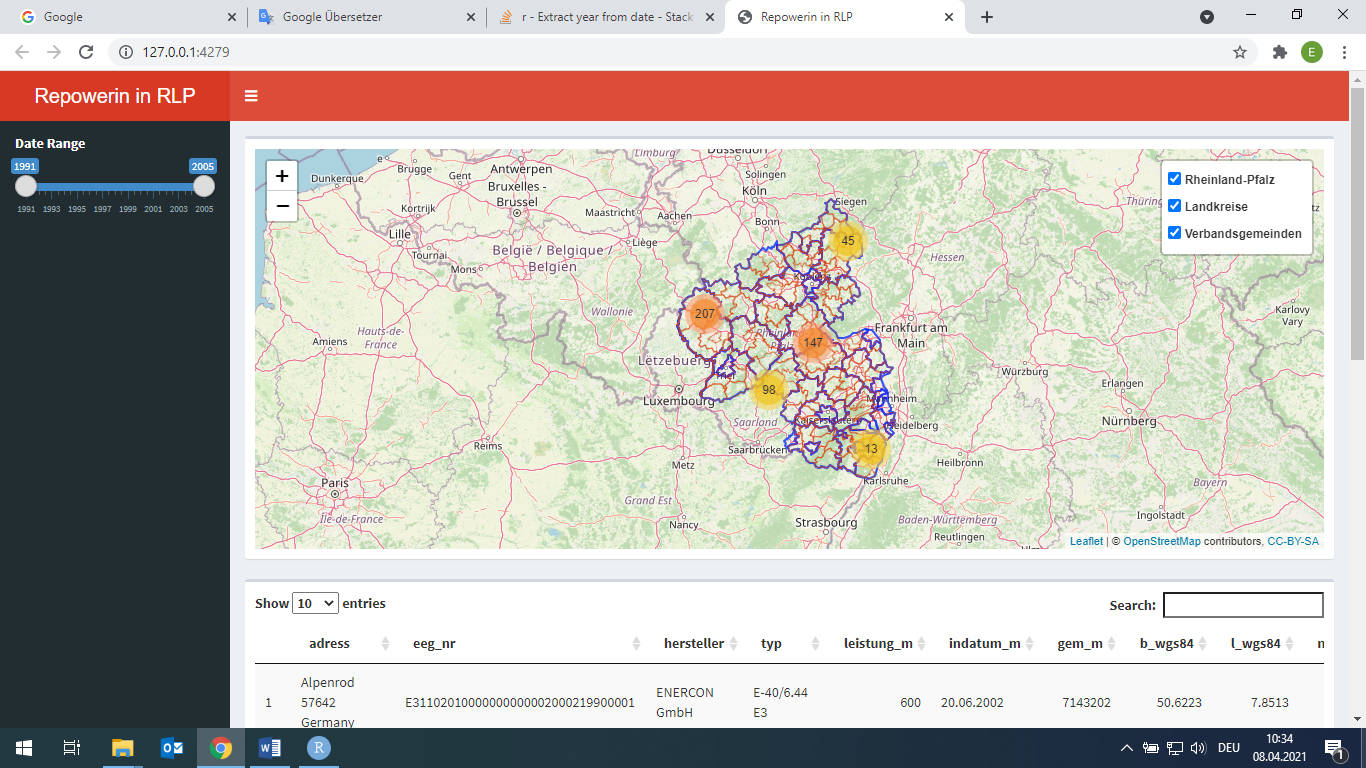
\includegraphics{images/repowering_image1.png}
\caption{Repowering application with date range slidebar in the upper
left corner, interactive Leaflet map with cluster options in the centre,
data table of selected WEPP at the bottom and check box to turn county
and municipality boarders on and off in the upper rigth corner}
\end{figure}

\begin{figure}
\centering
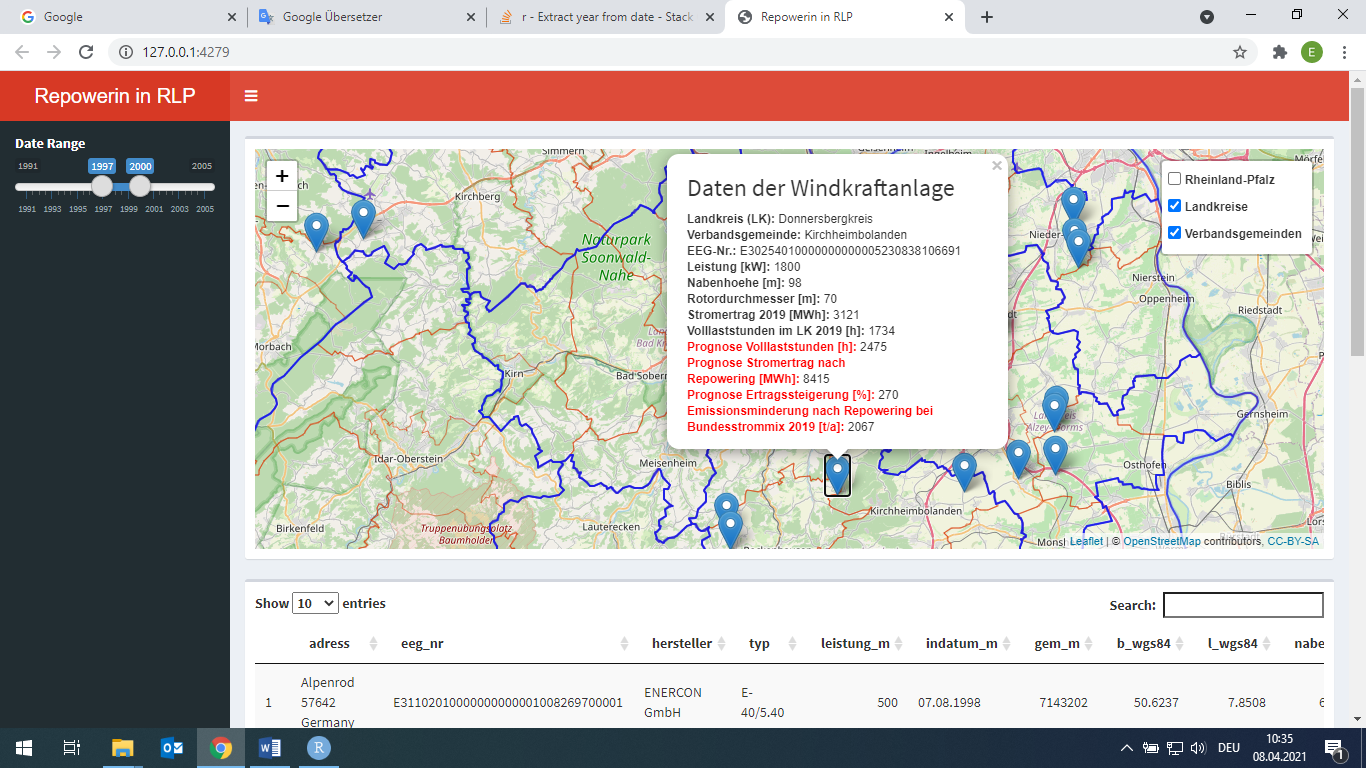
\includegraphics{images/repowering_image2.png}
\caption{Selected daterange from 1997 to 2000, zoom to county level and
view markers for each WEPP with popup of technical information and
forecasts in red letters in this case of a WEPP in Kirchheimbolanden of
the Donnersbergkreis}
\end{figure}

\hypertarget{sources}{%
\subsubsection{4. Sources}\label{sources}}

Chris Beely and Shitalkumar R. Sukhdeve (2018): Web Application
Development with R using Shiny - Third edition, Published by Packt
Publishing Ltd., \url{https://www.packtpub.com}

Yihui X. et al.~(2021): R Markdown Cookbook, CRC Press - Taylor and
Francis Group \url{https://www.crcpress.com}

Yihui X. et al.~(2019): R Markdown - The Definitve Guide, CRC Press -
Taylor and Francis Group \url{https://www.crcpress.com}

Landesregierung RLP (2021): Energiewende - Wind, Sonne Wasser,
\url{https://www.rlp.de/de/regierung/schwerpunkte/energiewende/\#:~:text=Rheinland\%2DPfalz\%20wird\%20bis\%20zum,einem\%20Viertel\%20entfallen.},
opened on the 10.03.2021

LKSG (2014): Landesgesetz zur Foerderung des Klimaschutzes vom 19.
August 2014,
\url{http://landesrecht.rlp.de/jportal/portal/t/onc/page/bsrlpprod.psml?pid=Dokumentanzeige\&showdoccase=1\&js_peid=Trefferliste\&documentnumber=1\&numberofresults=22\&fromdoctodoc=yes\&doc.id=jlr-KlimaSchGRPrahmen\&doc.part=X\&doc.price=0.0\&doc.hl=1},
opened on the 10.03.2021

Mac Kay JC (2009), Sustainable Energy - Without the hot air, UIT
Cambridge Ltd.

\end{document}
